		The input parameters for this problem are available in Table \ref{tab:10/7/1/7Table-1}
\begin{table}[H]


\caption{}
\label{tab:10/7/1/7Table-1}	
\end{table}
%
  If $\vec{O}$ lies on the  $x$-axis and is  equidistant from the points $\vec{A}$ and $\vec{B}$, 
\begin{align}
 \norm{\vec{O}-\vec{A}} &=
\norm{\vec{O}-\vec{B}} 
\\
 \implies \norm{\vec{O}-\vec{A}}^2 &=
\norm{\vec{O}-\vec{B}}^2 
\\
 \implies \norm{\vec{O}}^2-2{\vec{O}}^{\top}\vec{A} + \norm{\vec{A}}^2
	&= \norm{\vec{O}}^2-2{\vec{O}}^{\top}\vec{B} + \norm{\vec{B}}^2,
\end{align}
which can be simplified to obtain
  \begin{align}
	  \brak{\vec{A}-\vec{B}}^\top   \vec{O}&=\frac{\norm{\vec{A}}^2 -\norm{\vec{B}}^2 }{2}.
  \end{align}
  \begin{align}
  \because
   \vec{O} &=
    x\vec{e}_1,
  \end{align}
  \begin{align}
   x &=\frac{\norm{\vec{A}}^2 -\norm{\vec{B}}^2 }{2\brak{\vec{A}-\vec{B}}^{\top }\vec{e}_1.
}\label{eq:10/7/1/75}  
  \end{align}
  Substituting from \tabref{tab:10/7/1/7Table-1} in \eqref{eq:10/7/1/75},
 $x =  -7$.  Thus, 
		\begin{align}
\vec{O} = \myvec{ -7 \\ 0}.
		\end{align}
		See  
\figref{fig:10/7/1/7Fig1}.
\begin{figure}[H]
 \begin{center}
  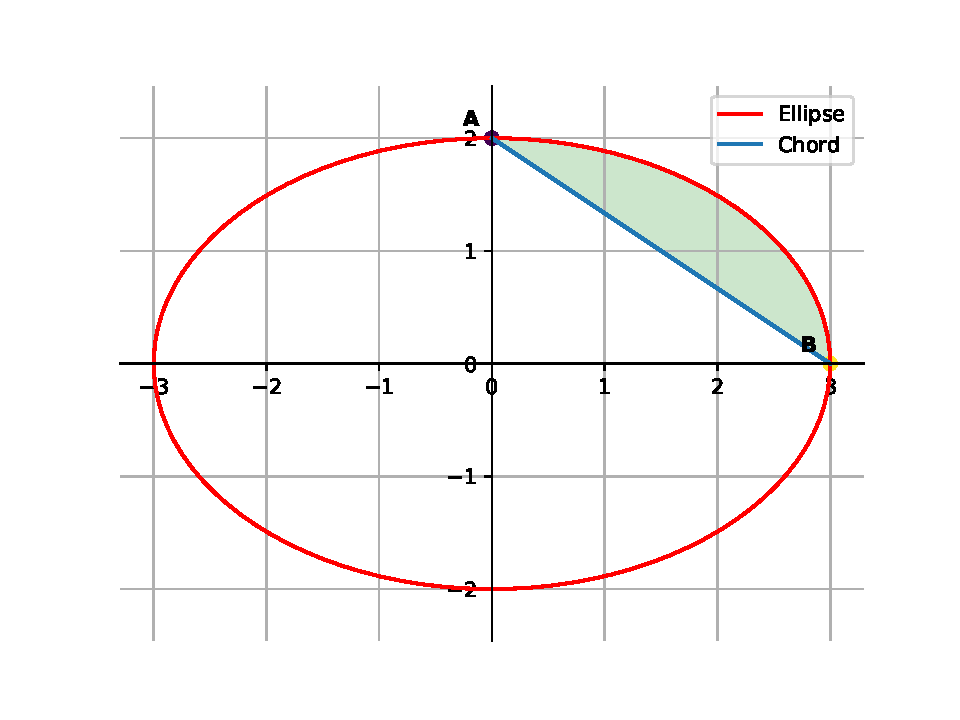
\includegraphics[width=0.75\columnwidth]{chapters/10/7/1/7/figs/fig.pdf}
 \end{center}
\caption{}
\label{fig:10/7/1/7Fig1}
\end{figure}

